\section{Method}
\label{sec:method}

\method{} augments the standard ReAct agent with three components: a failure detector, a memory store with hybrid retrieval, and a post-episode memory extractor. Figure~\ref{fig:architecture} illustrates the overall pipeline.

\begin{figure}[t]
    \centering
    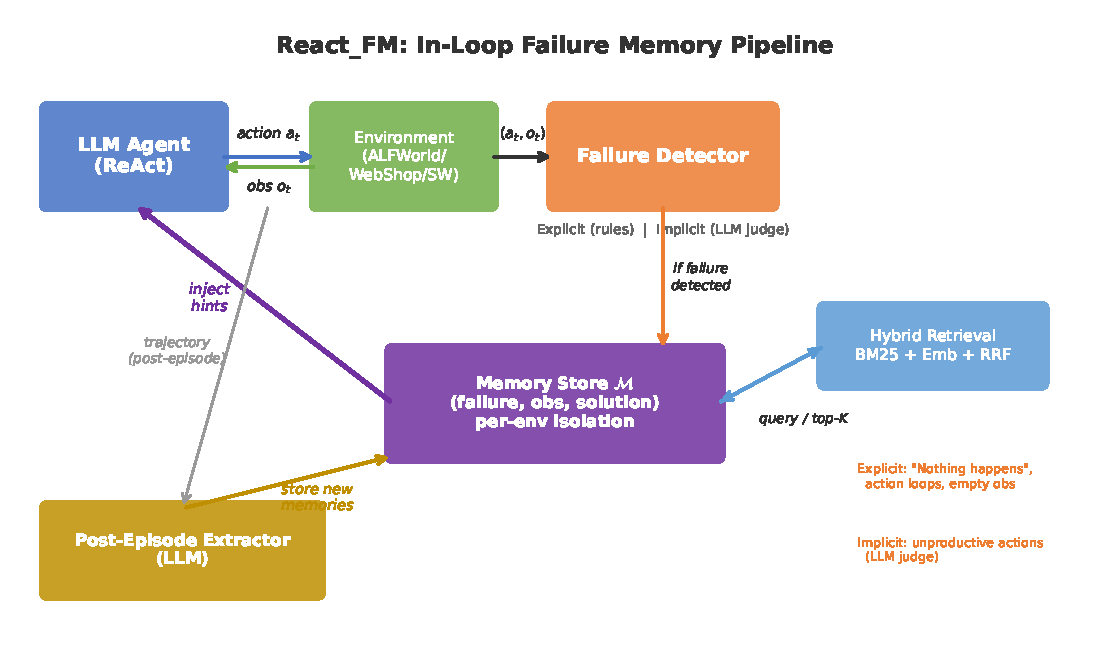
\includegraphics[width=\linewidth]{figures/architecture.pdf}
    \caption{Overview of \method{}. At each step, the failure detector monitors the action-observation pair for explicit failures (environment errors) and implicit failures (unproductive actions). Upon detecting a failure, relevant past experiences are retrieved via hybrid BM25-embedding retrieval and injected into the agent's prompt. After each episode, a separate LLM extracts failure-recovery pairs from the trajectory and stores them in the per-environment memory.}
    \label{fig:architecture}
\end{figure}

\subsection{Problem Formulation}
\label{sec:formulation}

We consider an agent interacting with a partially observable environment over discrete time steps. At step $t$, the agent observes $o_t$, selects action $a_t$ based on the history $h_t = (o_0, a_0, \ldots, o_{t-1}, a_{t-1}, o_t)$, and receives observation $o_{t+1}$. The agent maintains a memory store $\mathcal{M}$ containing failure-recovery entries from past episodes. The key question is \emph{when} and \emph{how} to leverage $\mathcal{M}$ during execution.

\subsection{Failure Detection}
\label{sec:detection}

When an agent interacts with an environment, failures manifest in two fundamentally different forms, analogous to how tool calls can fail in real-world agent systems:

\paragraph{Explicit Failures.} The environment directly signals that an action was invalid or had no effect. Examples include error messages (``Nothing happens'' in ALFWorld, ``No known action'' in ScienceWorld), empty observations, and action loops where the same action is repeated $k$ consecutive times ($k=3$) with no state change. These correspond to tool-call errors or API exceptions in practical agent systems. We detect them via zero-cost pattern matching rules.

\paragraph{Implicit Failures.} The action executes without error, but the outcome does not address the agent's intended goal. For example, an agent navigating to a location it has already visited, or picking up an object unrelated to the task---the environment responds normally, but no meaningful progress is made. These correspond to tool calls that return valid results that are nonetheless unhelpful. Detecting implicit failures requires understanding the \emph{intent} behind an action, which we accomplish through a lightweight LLM judge that evaluates whether each action-observation pair was \emph{productive}---whether the agent gained new information or changed the environment state toward the goal.

The two detection mechanisms are applied sequentially: explicit failure rules run first (zero cost), and the LLM judge is invoked only when no explicit failure is detected (amortized cost). This design ensures that the common, easy-to-detect failures are caught immediately, while subtle implicit failures are identified at moderate cost.

\subsection{Memory Store and Hybrid Retrieval}
\label{sec:retrieval}

A key design choice in \method{} is \emph{what} to store. Existing systems predominantly store success-derived knowledge: Reflexion stores free-text reflections summarizing what went wrong, ExpeL~\citep{zhao2024expel} extracts abstract insight rules by comparing successful and failed trajectories, and REMEMBERER~\citep{majumder2023rememberer} stores successful trajectory segments. These representations are \emph{abstract}---the agent must reason about how to apply a general insight (``always check if a container is open'') to a specific situation.

In contrast, \method{} stores structured \emph{failure-recovery pairs}:
\begin{equation}
    m = (\textit{failure\_action}, \textit{failure\_observation}, \textit{solution\_action}, \textit{task\_type}, \textit{env\_idx})
\end{equation}

This design offers three advantages. First, \textbf{retrieval precision}: failure scenarios are sparse and distinctive, providing natural anchors for retrieval---when the agent encounters a similar failure, the query (current failed action + observation) directly matches stored entries, unlike success trajectories which contain many routine steps that are hard to disambiguate. Second, \textbf{actionability}: the \texttt{solution\_action} field contains concrete corrective steps (\eg, ``open fridge 1 $\to$ take apple 1 from fridge 1'') that the agent can directly follow, reducing the reasoning burden compared to applying abstract rules. Third, \textbf{alignment with retrieval timing}: since retrieval is triggered by failures, storing failure-indexed memories creates a natural correspondence between the storage key and the retrieval query. Recent work on experiential reflective learning~\citep{chen2026erl} corroborates this design, finding that failure-derived heuristics substantially outperform success-derived ones for agent self-improvement.

Each environment maintains its own isolated memory store, ensuring that memories from one environment do not interfere with another, reflecting the fact that different environments have different objects, layouts, and solutions.

\paragraph{Hybrid Retrieval.} Given a detected failure with action $a$ and observation $o$, we construct query $q = a \| o$ and retrieve relevant entries using two complementary methods:

\begin{itemize}
    \item \textbf{BM25} (lexical): Ranks entries by term-frequency overlap, effective for matching specific object names and action patterns.
    \item \textbf{Sentence Embedding} (semantic): Computes cosine similarity using a pre-trained sentence transformer (all-MiniLM-L6-v2), capturing semantic similarity even when surface forms differ.
\end{itemize}

The two rankings are combined using Reciprocal Rank Fusion (RRF)~\citep{cormack2009reciprocal}:
\begin{equation}
    \text{RRF}(m) = \sum_{r \in \{r_{\text{BM25}}, r_{\text{emb}}\}} \frac{1}{k + r(m)}
\end{equation}
where $r(m)$ is the rank of entry $m$ in ranking $r$, and $k=60$ is the fusion constant. The top-$K$ entries (we use $K=3$) are returned.

\subsection{In-Loop Memory Injection}
\label{sec:injection}

When the failure detector triggers and retrieval returns relevant entries, the retrieved memories are formatted and appended to the agent's prompt before generating the next action:

\begin{quote}
\small\textit{You can refer to these past failure-recovery experiences to help decide your next action.}\\
\textit{- failure: take apple 1 from fridge 1, fix: open fridge 1 $\to$ take apple 1 from fridge 1}
\end{quote}

This injection is \emph{transient}: it appears only in the prompt immediately following the failure detection and is removed in subsequent steps, preventing prompt bloat.

\subsection{Post-Episode Memory Extraction}
\label{sec:extraction}

After each episode, a separate LLM (the extractor) analyzes the trajectory to identify failure-recovery patterns: sequences where an action fails, the agent takes corrective steps, and the original goal is eventually achieved. These are stored as structured $(failure\_action, failure\_observation, solution\_action)$ triples. The extractor is prompted with few-shot examples to ensure consistent output format.

This extraction step runs \emph{after} each episode regardless of success or failure, enabling the agent to learn from both recovered and unrecovered failures.

\subsection{Overall Algorithm}

Algorithm~\ref{alg:reactfm} summarizes the \method{} procedure for a single episode.

\begin{algorithm}[t]
\caption{\method{} Episode Execution}
\label{alg:reactfm}
\begin{algorithmic}[1]
\REQUIRE Environment $\mathcal{E}$, memory store $\mathcal{M}$, max steps $T$
\STATE $o_0, \textit{task\_type} \leftarrow \mathcal{E}.\text{reset}()$
\STATE $h \leftarrow [o_0]$; $\textit{hints} \leftarrow \emptyset$
\FOR{$t = 0$ to $T-1$}
    \STATE $a_t \leftarrow \text{LLM}(h, \textit{hints})$ \COMMENT{Generate action}
    \STATE $\textit{hints} \leftarrow \emptyset$ \COMMENT{Clear transient injection}
    \STATE $o_{t+1} \leftarrow \mathcal{E}.\text{step}(a_t)$
    \IF{$\text{ExplicitFail}(o_{t+1})$ \OR $\text{ImplicitFail}(a_t, o_{t+1})$}
        \STATE $\textit{hints} \leftarrow \mathcal{M}.\text{retrieve}(a_t, o_{t+1})$ \COMMENT{RRF retrieval}
    \ENDIF
    \STATE $h \leftarrow h \cup \{(a_t, o_{t+1})\}$
    \IF{$\mathcal{E}.\text{done}()$}
        \STATE \textbf{break}
    \ENDIF
\ENDFOR
\STATE $\text{pairs} \leftarrow \text{Extract}(h)$ \COMMENT{LLM extractor}
\STATE $\mathcal{M}.\text{add}(\text{pairs})$ \COMMENT{Store for future epochs}
\end{algorithmic}
\end{algorithm}
